\section{Proofs of Proposition 3.1}
\label{app_proof}

\begin{proof}
We write simplified updates of HEPi and $\text{MPNN}$ + $\text{VN}_\text{local}$ as follows,

{\bf HEPi}:
\begin{equation}
\begin{aligned}
\mathbf{f}_v^{\text{obj}, (l+1)} &= \mathbf{f}_v^{\text{obj},(l)}  + \sigma \left(W^{(l)}_o \sum_{u \in N(v)_\text{obj}} k(\cdot, \cdot; \theta_\text{obj-obj}) \mathbf{f}_u^{\text{obj},(l)} \right), \quad v \in \gV_\text{obj}, \\
\mathbf{f}_v^{\text{act, new}, (l+1)} &=  \mathbf{f}_v^{\text{act}, (l)} + \sigma \left(W_a^{\text{local}, (l)} \sum_{w \in N(v)_\text{act}} k(\cdot, \cdot; \theta_\text{act-act}) \mathbf{f}_w^{\text{act}, (l)} \right), \quad v \in \gV_\text{act}, \\
\mathbf{f}_v^{\text{act}, (l+1)} &= \mathbf{f}_v^{\text{act, new}, (l+1)} +  \mathbf{f}_v^{\text{act},(l)} + \sigma \left(W_{a}^{(l)} \sum_{{\color{red}u \in {\cal V}_\text{obj}}} k(\cdot, \cdot; \theta_\text{obj-act}) \mathbf{f}_u^{\text{obj, L}} \right), \quad v \in \gV_\text{act}.
\end{aligned}
\label{app_hepi_update}
\end{equation}

where $\sigma$ is activation function, and $W^{(l)}$ is the weight at layer $l$. Note that the object nodes are updated through $L$ layers.

{\bf $\text{MPNN}$ + $\text{VN}_\text{local}$}:

\begin{equation}
\begin{aligned}
\mathbf{f}_v^{\text{obj}, (l+1)} &= \mathbf{f}_v^{\text{obj},(l)}  +\sigma \left(W^{(l)}_o \sum_{u \in N(v)_\text{obj}} k(\cdot, \cdot; \theta_\text{obj-obj}) \mathbf{f}_u^{\text{obj},(l)} \right), \quad v \in \gV_\text{obj}, \\
\mathbf{f}_v^{\text{act, new}, (l+1)} &=  \mathbf{f}_v^{\text{act}, (l)} + \sigma \left(W_a^{\text{local}, (l)}  \sum_{w \in N(v)_\text{act}} k(\cdot, \cdot; \theta_\text{act-act}) \mathbf{f}_w^{\text{act}, (l)} \right), \quad v \in \gV_\text{act}, \\
\mathbf{f}_v^{\text{act}, (l+1)} &= \mathbf{f}_v^{\text{act, new}, (l+1)} +  \mathbf{f}_v^{\text{act},(l)} + \sigma \left(W_{a}^{(l)} \sum_{{\color{red}u \in N_k(v)_\text{obj}}} k(\cdot, \cdot; \theta_\text{obj-act}) \mathbf{f}_u^{\text{obj}, L} \right), \quad v \in \gV_\text{act}.
\end{aligned}
\label{app_mpnn_local_update}
\end{equation}

As seen, the main difference between HEPi and $\text{MPNN}$ + $\text{VN}_\text{local}$ is at treating the actuator nodes as VN nodes as in $\text{MPNN}$ + $\text{VN}_\text{G}$ or normal graph nodes with k-NN connections.

For HEPi, the actuator nodes are updated through every object node as in the third equation in Eq.~\ref{app_hepi_update}. Explicitly, we compute its Jacobian w.r.t object nodes as
\begin{equation}
\begin{aligned}
    \frac{\partial \mathbf{f}_v^{\text{act}, (l+1)}}
    {\partial \mathbf{f}_u^{\text{obj}, L}} =& 2\nabla  \mathbf{f}_v^{\text{act}, (l)}  + \sigma'(z_v^{\text{local},(l)}) W_a^{\text{local}, (l)} \sum_{w \in N(v)_\text{act}}k(x_v,x_w; \theta_\text{act-act}) \nabla  \mathbf{f}_v^{\text{act}, (l)} \\
    &+ \sigma'(z_v^{(l)}) W_{a}^{(l)} k(x_v,x_u; \theta_\text{obj-act}) \\
\end{aligned}
\label{app_jacobian}
\end{equation}
% where we let 
% \begin{align*}
%     z_v^{(l)} &= \left(W_{a}^{(l)} \sum_{{\color{red}u \in {\cal V}_\text{obj}}} k(\cdot, \cdot; \theta_\text{obj-act}) \mathbf{f}_u^{\text{obj}, L} \right), \\
%     z_v^{\text{local},(l)} &= \left(W_a^{\text{local}, (l)} \sum_{w \in N(v)_\text{act}} k(\cdot, \cdot; \theta_\text{act-act}) \mathbf{f}_w^{\text{act}, (l)} \right)
% \end{align*}
with $z_v^{(l)}$ = $W_{a}^{(l)} \sum_{{\color{red}u \in {\cal V}_\text{obj}}} k(\cdot, \cdot; \theta_\text{obj-act}) \mathbf{f}_u^{\text{obj}, L} $ and $z_v^{\text{local},(l)}$=$W_a^{\text{local}, (l)} \sum_{w \in N(v)_\text{act}} k(\cdot, \cdot; \theta_\text{act-act}) \mathbf{f}_w^{\text{act}, (l)} $ be the evaluation of the argument of the function $\sigma$. This shows that any object node can exchange information with the actuator nodes after a single layer of the object-actuator update.
%actuator-actuator update.

For $\text{MPNN}$ + $\text{VN}_\text{local}$, if an actuator node $v$ and an object node $u$ are more than 2-hops distant from each other, the message from node $u$ sent to $v$ will arrive either through another actuator node (via actuator-actuator updates) or through a node where the $k$-NN connections of those actuator nodes overlap (depicted in Figure~\ref{fig:appendix_theory}). However, in both cases, the Jacobian at the actuator node $v$ becomes independent of the feature at the object node $u$, i.e., it can only receive a homogeneous value from the VN (overlapping node or other actuator node) \citep{southern2024understanding}. Consequently, the policy could fail to predict relevant actions in response to changes at the object node $u$.
\end{proof}

% For $\text{MPNN}$ + $\text{VN}_\text{local}$, if actuator node $v$ and object node $u$ are more than 2-hop distant from each other, then message from node $u$ sent to $v$ will arrive through the other actuator node, i.e. the actuator-actuator updates, only if the k-NN connections of those actuator nodes are overlapping. 
% More specifically, in this case, we can compute the Jacobian similar to Eq.~\ref{app_jacobian}.  In other cases, if actuator node $v$ and object node $u$ are more than 2-hop distant from each other 
% and the k-NN connections of those actuator nodes are not overlapping. In this case, the Jacobian at the actuator node $v$ is independent of feature at the object node $u$. This interpretation is depicted in Figure \ref{fig:appendix_theory}. In other words, the actuators only
% receive homogeneous values from object node \citep{southern2024understanding}, therefore the policy could fail to predict relevant actions to changes at object node $u$.


\paragraph{Related Work for Oversquashing in Graph Neural Networks}

Transformers \citep{attention} can be viewed as fully connected GNNs under the \gls{mpnn} framework \citep{battaglia2018relational}, since self-attention can be seen as a mechanism to aggregate messages from its neighbors. While GNNs offer efficient local information processing with linear complexity $\mathcal{O}(|V| + |E|)$, they struggle with \emph{over-squashing}, limiting their ability to propagate information across distant nodes \citep{oversquashing}. In contrast, Transformers, by being fully connected, allow every node to exchange information with all others, making them well-suited for tasks requiring global information aggregation, though at a higher quadratic complexity $\mathcal{O}(|V|^2)$.

Recent studies have shown that introducing virtual nodes (VN) in GNNs can mitigate the over-squashing issue by facilitating long-range information exchange while retaining the lower complexity of GNNs \citep{oversquashing, pmlr-v202-cai23b, rosenbluth2024distinguished}. Our \model builds on this insight, treating actuators as virtual nodes to enable efficient global information aggregation from object nodes, as shown in Figure~\ref{fig:hepi_diagram}.

\begin{figure*}[t]
    \centering
    \begin{subfigure}[b]{0.3\linewidth}
        \centering
        \includegraphics[width=\textwidth]{ICLR_2025/Figures/appx_theory/Knn_overlap.pdf}
        \caption{Overlapping node.}
    \end{subfigure}
    \hspace{1cm}
    \begin{subfigure}[b]{0.3\linewidth}
        \centering
        \includegraphics[width=\textwidth]{ICLR_2025/Figures/appx_theory/Knn_non_overlap.pdf}
        \caption{No overlapping node.}
    \end{subfigure}
    \caption{
    Demonstration of graph with overlapping and non-overlapping nodes. Actuator nodes are in red, object nodes are in either white or orange.
    }
    \label{fig:appendix_theory}
\end{figure*}


%%%%

\section{Tasks Details}
\label{appx:task_details}

Here, we provide detailed specifications for each of the \rebuttal{seven} manipulation tasks introduced in the main paper.



\subsection{Rigid-Sliding}
The goal of the Rigid-Sliding task is to control an object using a suction gripper and slide it on a 2D plane to a desired target position and orientation. The agent controls the object’s linear velocity $v$ and angular velocity $\omega$ in the yaw direction. 

\begin{figure*}[htb]
    \centering
    \begin{minipage}{0.19\textwidth}
            \centering
            \includegraphics[width=\textwidth]{ICLR_2025/Figures/appx_tasks/rigid-sliding/ris1.png}
    \end{minipage}
    \begin{minipage}{0.19\textwidth}
            \centering
            \includegraphics[width=\textwidth]{ICLR_2025/Figures/appx_tasks/rigid-sliding/ris2.png}
    \end{minipage}
    \begin{minipage}{0.19\textwidth}
            \centering
            \includegraphics[width=\textwidth]{ICLR_2025/Figures/appx_tasks/rigid-sliding/ris3.png}
    \end{minipage}
    \begin{minipage}{0.19\textwidth}
            \centering
            \includegraphics[width=\textwidth]{ICLR_2025/Figures/appx_tasks/rigid-sliding/ris4.png}
    \end{minipage}
    % \begin{minipage}{0.19\textwidth}
    %         \centering
    %         \includegraphics[width=\textwidth]{ICLR_2025/Figures/appx_tasks/rigid-sliding/ris5.png}
    % \end{minipage}
    \begin{minipage}{0.19\textwidth}
            \centering
            \includegraphics[width=\textwidth]{ICLR_2025/Figures/appx_tasks/rigid-sliding/ris6.png}
    \end{minipage}

    \caption{
    Example trajectory of Rigid Sliding task.
    }
    \label{fig:appendix_ris_vis}
\end{figure*}

\paragraph{Input and Output}
The input space for each node includes:
\begin{itemize}
    \item Gripper nodes: \texttt{node\_type}, position $\mathbf{p}_a$, velocity $\mathbf{v}_a$, angular velocity $\omega_a$.
    \item Object nodes: \texttt{node\_type}, position $\mathbf{p}_o$, distance to target $d_{\text{target}}$.
\end{itemize}

The output consists of the gripper's linear velocity $v_a$ and a vector from which the angular velocity $\omega_a$ is derived. Specifically, the vector is decomposed into its parallel and tangential components with respect to the position vector $\mathbf{r}$, where $\mathbf{v}_{\parallel} = \left( \frac{\mathbf{v} \cdot \mathbf{r}}{\|\mathbf{r}\|^2} \right) \mathbf{r}$ and $\mathbf{v}_{\perp} = \mathbf{v} - \mathbf{v}_{\parallel}$. The angular velocity is then computed as $\omega_a = \frac{\mathbf{r} \times \mathbf{v}_{\perp}}{\|\mathbf{r}\|^2}$.

\paragraph{Sample Space}
\begin{itemize}
    \item Initial pose: $(x, y, \theta_\text{yaw}) \in [-1, 1]^2 \times [-\pi, \pi]$.
    \item Target pose: $\theta_\text{yaw} \in [-\pi, \pi]$.
\end{itemize}

\paragraph{Reward Function}
The reward consists of multiple sub-rewards:

\begin{itemize}
    \item \textbf{Distance to goal}: \[
        R_\text{goal} = \lVert \mathbf{p}_o - \mathbf{p}_{goal} \rVert
    \]
    where $\mathbf{p}_o$ is the object position and $\mathbf{p}_{goal}$ is the target position.
    \item \textbf{Rotation distance}: \[
        R_\text{rotation} = \texttt{quat\_diff}(\mathbf{r}_o, \mathbf{r}_{goal})
    \]
    where $\mathbf{r}_o$ and $\mathbf{r}_{goal}$ are the object and goal orientations in quaternion.
    \item \textbf{Object velocity penalty}: \[
        V_{\text{object}} = v_{\text{angular}} + v_{\text{linear}}
    \]
    where $v_{\text{angular}}$ and $v_{\text{linear}}$ are the angular and linear velocities of the object.
    \item \textbf{Action rate penalty}: \[
A_{\text{actions}} = \sqrt{a_i - a_{i-1}}
\]
where $a_i$ and $a_{i-1}$ are the actions at the current and previous time steps.

\end{itemize}

The total time-dependent reward with $T=100$ is:
\begin{equation*}
    R_\text{tot} = \begin{cases}
        -0.8 R_\text{goal} - 0.4 R_\text{rotation} - 0.1 V_{\text{object}} - 0.002 A_{\text{actions}}, & t < T-2, \\
        -4.0 R_\text{goal} - 2.0 R_\text{rotation} - 0.1 V_{\text{object}} - 0.002 A_{\text{actions}}, & t \geq T-2.
    \end{cases}
\end{equation*}

% {\color{blue}

\subsection{Rigid-Pushing}
The goal of the Rigid-Pushing task is to control an object using a rod and push it on a 2D plane to a desired target position and orientation. The agent controls the object’s linear velocity $v$. 

\begin{figure*}[htb]
    \centering
    \begin{minipage}{0.19\textwidth}
            \centering
            \includegraphics[width=\textwidth]{ICLR_2025/Figures/appx_tasks/rigid-pushing/rp-1.png}
    \end{minipage}
    \begin{minipage}{0.19\textwidth}
            \centering
            \includegraphics[width=\textwidth]{ICLR_2025/Figures/appx_tasks/rigid-pushing/rp-2.png}
    \end{minipage}
    \begin{minipage}{0.19\textwidth}
            \centering
            \includegraphics[width=\textwidth]{ICLR_2025/Figures/appx_tasks/rigid-pushing/rp-3.png}
    \end{minipage}
    \begin{minipage}{0.19\textwidth}
            \centering
            \includegraphics[width=\textwidth]{ICLR_2025/Figures/appx_tasks/rigid-pushing/rp-4.png}
    \end{minipage}
    \begin{minipage}{0.19\textwidth}
            \centering
            \includegraphics[width=\textwidth]{ICLR_2025/Figures/appx_tasks/rigid-pushing/rp-5.png}
    \end{minipage}

    \caption{
    \rebuttal{Example trajectory of Rigid Pushing task.}
    }
    \label{fig:appendix_rigid_pushing_vis}
\end{figure*}

\paragraph{Input and Output}
The input space for each node includes:
\begin{itemize}
    \item Gripper nodes: \texttt{node\_type}, position $\mathbf{p}_a$, velocity $\mathbf{v}_a$, angular velocity $\omega_a$.
    \item Object nodes: \texttt{node\_type}, position $\mathbf{p}_o$, distance to target $d_{\text{target}}$, and object's linear velocity $\mathbf{v}_{\text{o}}$.
\end{itemize}

The output consists of the actuator's linear velocity $v_a$.

\paragraph{Sample Space}
\begin{itemize}
    \item Initial pose: $(x, y, \theta_\text{yaw}) \in [-0.5, 0.5]^2 \times [-\pi, \pi]$.
    \item Target pose: $\theta_\text{yaw} \in [-\pi, \pi]$.
\end{itemize}

\paragraph{Reward Function}
The reward consists of multiple sub-rewards:

\begin{itemize}
    \item \textbf{Distance to goal}: \[
        R_\text{goal} = \lVert \mathbf{p}_o - \mathbf{p}_{goal} \rVert
    \]
    where $\mathbf{p}_o$ is the object position and $\mathbf{p}_{goal}$ is the target position.
    \item \textbf{Rotation distance}: \[
        R_\text{rotation} = \texttt{quat\_diff}(\mathbf{r}_o, \mathbf{r}_{goal})
    \]
    where $\mathbf{r}_o$ and $\mathbf{r}_{goal}$ are the object and goal orientations in quaternion.
    \item \textbf{Distance to object}: \[
        R_\text{object} = \lVert \mathbf{p}_o - \mathbf{p}_{actuator} \rVert,
    \]
    encouraging the rod (actuator) to stay close to the object during pushing.

\end{itemize}

The total time-dependent reward with $T=100$ is:
\begin{equation*}
    R_\text{tot} = \begin{cases}
        -0.8 R_\text{goal} - 0.08 R_\text{rotation} - 0.2 R_\text{object}, & t < T-5, \\
        -8.0 R_\text{goal} - 0.8 R_\text{rotation} - 0.2 R_\text{object}, & t \geq T-5.
    \end{cases}
\end{equation*}
% }

\subsection{Rigid-Insertion}

The Rigid-Insertion task extends Rigid-Sliding to 3D, where the agent must control both linear and angular velocities to move an object along the $z$-axis and insert it into a hole. The state space includes $(x, y, z, \theta)$, and precise alignment is required near the hole before sliding and rotating the object into place.

\begin{figure*}[htb]
    \centering
    \begin{minipage}{0.19\textwidth}
            \centering
            \includegraphics[width=\textwidth]{ICLR_2025/Figures/appx_tasks/rigid-insertion/ri1.png}
    \end{minipage}
    \begin{minipage}{0.19\textwidth}
            \centering
            \includegraphics[width=\textwidth]{ICLR_2025/Figures/appx_tasks/rigid-insertion/ri2.png}
    \end{minipage}
    \begin{minipage}{0.19\textwidth}
            \centering
            \includegraphics[width=\textwidth]{ICLR_2025/Figures/appx_tasks/rigid-insertion/ri4.png}
    \end{minipage}
    \begin{minipage}{0.19\textwidth}
            \centering
            \includegraphics[width=\textwidth]{ICLR_2025/Figures/appx_tasks/rigid-insertion/ri5.png}
    \end{minipage}
    \begin{minipage}{0.19\textwidth}
            \centering
            \includegraphics[width=\textwidth]{ICLR_2025/Figures/appx_tasks/rigid-insertion/ri6.png}
    \end{minipage}

    \caption{
    Example trajectory of Rigid Insertion task.
    }
    \label{fig:appendix_ri_vis}
\end{figure*}

\paragraph{Input and Output}
The input space for each node includes:
\begin{itemize}
    \item Gripper nodes: \texttt{node\_type}, position $\mathbf{p}_a$, velocity $\mathbf{v}_a$, angular velocity $\omega_a$.
    \item Object nodes: \texttt{node\_type}, position $\mathbf{p}_o$, distance to target $d_{\text{target}}$.
\end{itemize}

The output consists of the gripper's linear velocity $v_a$ and a vector from which the angular velocity $\omega_a$ is derived. Specifically, the vector is decomposed into its parallel and tangential components with respect to the position vector $\mathbf{r}$, where $\mathbf{v}_{\parallel} = \left( \frac{\mathbf{v} \cdot \mathbf{r}}{\|\mathbf{r}\|^2} \right) \mathbf{r}$ and $\mathbf{v}_{\perp} = \mathbf{v} - \mathbf{v}_{\parallel}$. The angular velocity is then computed as $\omega_a = \frac{\mathbf{r} \times \mathbf{v}_{\perp}}{\|\mathbf{r}\|^2}$. 

\paragraph{Sample Space}
\begin{itemize}
    \item Initial pose: $(x, y, z, \theta_\text{yaw}) \in [-1, 1]^2 \times [0, 0.5] \times [-\pi, \pi]$.
    \item Target pose: $\theta_\text{yaw} \in [-\pi, \pi]$.
\end{itemize}

\paragraph{Reward Function}
The total reward consists of the following sub-rewards:
\begin{itemize}
    \item \textbf{Distance to goal}:
    \[
    R_\text{goal} = \lVert \mathbf{p}_o - \mathbf{p}_{goal} \rVert
    \]
    where $\mathbf{p}_o$ is the object's position, and $\mathbf{p}_{goal}$ is the target position.
    
    \item \textbf{Rotation distance}: \[
        R_\text{rotation} = \texttt{quat\_diff}(\mathbf{r}_o, \mathbf{r}_{goal})
    \]
    where $\mathbf{r}_o$ and $\mathbf{r}_{goal}$ are the object and goal orientations in quaternion.

    \item \textbf{Distance along $z$-axis}:
    \[
    R_\text{goal, z} = \lVert \mathbf{p}_{o, z} - \mathbf{p}_{goal, z} \rVert
    \]
    where $\mathbf{p}_{o, z}$ and $\mathbf{p}_{goal, z}$ represent the positions along the $z$-axis.
\end{itemize}

The total time-dependent reward with $T=100$ is defined as:
\[
R_\text{tot} = \begin{cases}
    - 0.8 R_\text{goal} - 2.0 R_\text{rotation} - 0.4 R_\text{goal, z}, & t < T-2, \\
    - 4.0 R_\text{goal} - 4.0 R_\text{rotation} - 0.4 R_\text{goal, z}, & t \geq T-2.
\end{cases}
\]

\subsection{Rigid-Insertion-Two-Agents}
The Rigid-Insertion-Two-Agents task extends Rigid-Insertion into 3D with two linear actuators controlling the object. The object's initial position and the target are sampled from the upper hemisphere. Control is limited to linear velocities along two axes, simplifying the task for stability in physical systems.

\begin{figure*}[htb]
    \centering
    \begin{minipage}{0.19\textwidth}
            \centering
            \includegraphics[width=\textwidth]{ICLR_2025/Figures/appx_tasks/rigid-insertion-3d/ri3d1.png}
    \end{minipage}
    \begin{minipage}{0.19\textwidth}
            \centering
            \includegraphics[width=\textwidth]{ICLR_2025/Figures/appx_tasks/rigid-insertion-3d/ri3d2.png}
    \end{minipage}
    \begin{minipage}{0.19\textwidth}
            \centering
            \includegraphics[width=\textwidth]{ICLR_2025/Figures/appx_tasks/rigid-insertion-3d/ri3d3.png}
    \end{minipage}
    % \begin{minipage}{0.19\textwidth}
    %         \centering
    %         \includegraphics[width=\textwidth]{ICLR_2025/Figures/appx_tasks/rigid-insertion-3d/ri3d4.png}
    % \end{minipage}
    \begin{minipage}{0.19\textwidth}
            \centering
            \includegraphics[width=\textwidth]{ICLR_2025/Figures/appx_tasks/rigid-insertion-3d/ri3d5.png}
    \end{minipage}
    \begin{minipage}{0.19\textwidth}
            \centering
            \includegraphics[width=\textwidth]{ICLR_2025/Figures/appx_tasks/rigid-insertion-3d/ri3d6.png}
    \end{minipage}

    \caption{
    Example trajectory of Rigid Insertion with Two Agents task.
    }
    \label{fig:appendix_ri3d_vis}
\end{figure*}

\paragraph{Input and Output}
The input space for each node includes:
\begin{itemize}
    \item Gripper nodes: \texttt{node\_type}, position $\mathbf{p}_a$, velocity $\mathbf{v}_a$.
    \item Object nodes: \texttt{node\_type}, position $\mathbf{p}_o$, distance to target $d_{\text{target}}$.
\end{itemize}

The output consists of the gripper's velocities; however, only the linear velocity $v_a$. 

\paragraph{Sample Space}
\begin{itemize}
    \item Initial pose: translate in $x \in [0.25, 0.75], y \in [-0.75, 0.75], z \in [0.5, 1.25]$, and rotate around its own axis between $[-\pi, \pi]$.
    \item Target pose: $(\theta_{pich}, \theta_{yaw}) \in [-\pi / 2, 0] \times [-\pi, \pi]$. These samples lie in an upper-hemisphere when rotating a unit-vector $[1, 0, 0]^T$ - an initial pose of the target placement, as shown in Figure~\ref{fig:ri3d-sample-space}.
    \begin{figure*}[ht]
        \centering
        \includegraphics[width=0.32\linewidth]{ICLR_2025/Figures/appx_tasks/rigid-insertion-3d/rigid-insertion-two-agents-sample-space.png}
        \caption{Sample space of the Rigid-Insertion-Two-Agents task.}
    
        \label{fig:ri3d-sample-space}
    \end{figure*}
\end{itemize}

\paragraph{Reward Function}
The total reward consists of the following components:
\begin{itemize}
    \item \textbf{Distance to goal}:
    \[
    R_\text{goal} = \lVert \mathbf{p}_o - \mathbf{p}_{goal} \rVert
    \]
    where $\mathbf{p}_o$ is the object's position, and $\mathbf{p}_{goal}$ is the target position.
    
    \item \textbf{Rotation distance}: \[
        R_\text{rotation} = \texttt{quat\_diff}(\mathbf{r}_o, \mathbf{r}_{goal})
    \]
    where $\mathbf{r}_o$ and $\mathbf{r}_{goal}$ are the object and goal orientations in quaternion.
\end{itemize}
The time-dependent reward with $T=100$ is defined as:
\[
R_\text{tot} = \begin{cases}
    - 0.8 R_\text{goal} - 0.08 R_\text{rotation}, & t < T-2, \\
    - 4.0 R_\text{goal} - 0.6 R_\text{rotation}, & t \geq T-2.
\end{cases}
\]

\subsection{Rope-Closing}
In Rope-Closing, two actuators manipulate the endpoints of a deformable rope in a 2D plane, with the goal of wrapping the rope around a cylindrical object and closing the loop. The rope is segmented into 40 links, with each node representing the pose of a link.

\begin{figure*}[htb]
    \centering
    \begin{minipage}{0.19\textwidth}
            \centering
            \includegraphics[width=\textwidth]{ICLR_2025/Figures/appx_tasks/rope-closing/rs1.png}
    \end{minipage}
    \begin{minipage}{0.19\textwidth}
            \centering
            \includegraphics[width=\textwidth]{ICLR_2025/Figures/appx_tasks/rope-closing/rs2.png}
    \end{minipage}
    % \begin{minipage}{0.19\textwidth}
    %         \centering
    %         \includegraphics[width=\textwidth]{ICLR_2025/Figures/appx_tasks/rope-closing/rs3.png}
    % \end{minipage}
    \begin{minipage}{0.19\textwidth}
            \centering
            \includegraphics[width=\textwidth]{ICLR_2025/Figures/appx_tasks/rope-closing/rs4.png}
    \end{minipage}
    \begin{minipage}{0.19\textwidth}
            \centering
            \includegraphics[width=\textwidth]{ICLR_2025/Figures/appx_tasks/rope-closing/rs5.png}
    \end{minipage}
    \begin{minipage}{0.19\textwidth}
            \centering
            \includegraphics[width=\textwidth]{ICLR_2025/Figures/appx_tasks/rope-closing/rs6.png}
    \end{minipage}

    \caption{
    Example trajectory of Rope Closing task.
    }
    \label{fig:appendix_rc_vis}
\end{figure*}

\paragraph{Input and Output}
The input space for each node includes:
\begin{itemize}
    \item Gripper nodes: \texttt{node\_type}, position $\mathbf{p}_a$, velocity $\mathbf{v}_a$.
    \item Object nodes: \texttt{node\_type}, position $\mathbf{p}_o$, velocity $\mathbf{v}_o$, distance to target $d_{\text{target}}$.
\end{itemize}
The output consists of the gripper's linear velocity $v_a$. 

\paragraph{Sample Space}
In this task, the rope starts in a straight configuration, and only the mid-point position is sampled, with the rope constrained to move accordingly,
\begin{itemize}
    \item Initial rope mid-point: $\theta_\text{yaw} \in [-\pi / 4, \pi / 4]$.
    \item Target cylinder: $(x, y, \theta_\text{yaw}) \in [-0.5, 0.5]^2 \times [-\pi, \pi]$.
\end{itemize}

\paragraph{Reward Function}
The total reward consists of:
\begin{itemize}
    \item \textbf{Rope closing reward}:
    \[
    R_{\text{rope closing}} = \| (x_{\text{gripper}_0}, y_{\text{gripper}_0}) - (x_{\text{gripper}_1}, y_{\text{gripper}_1}) \|
    \]
    \item \textbf{Center wrapping reward}:
    \[
    R_\text{wrapping} = \| (x_{\text{hanger}}, y_{\text{hanger}}) - (\mathbf{C}_{\text{rope}, x}, \mathbf{C}_{\text{rope}, y}) \|
    \]
    where $\mathbf{C}_{\text{rope}}$ is the center of the rope:
    \[
    \mathbf{C}_{\text{rope}} = \frac{1}{n_{\text{nodes}}} \sum_{i=1}^{n_{\text{nodes}}} \mathbf{p}_{\text{node}_i}
    \]
    \item \textbf{Link velocity penalty}:
    \[
    V_{\text{links}} = \frac{1}{n_{\text{links}}} \sum_{i=1}^{n_{\text{links}}} \| v_{\text{link}_i} \|
    \]
    \item \textbf{Action rate penalty}:
    \[
    A_{\text{actions}} = \sqrt{a_{i} - a_{i-1}}
    \]
\end{itemize}

The total time-dependent reward with $T=200$ is defined as:
\[
R_\text{tot} = \begin{cases}
    - 0.8 R_\text{wrapping} - 0.01 V_{\text{links}} - 0.001 A_{\text{actions}}, & t < T-20, \\
    - 2.0 R_\text{rope closing} - 0.8 R_\text{wrapping} - 0.01 V_{\text{links}} - 0.001 A_{\text{actions}}, & t \geq T-20.
\end{cases}
\]

\subsection{Rope-Shaping}
This task requires the rope to form a specific shape (e.g., a ``W") to a desired orientation by controlling the actuators. The rope is segmented into 80 links, with each node representing the pose of a link.

\begin{figure*}[htb]
    \centering
    \begin{minipage}{0.19\textwidth}
            \centering
            \includegraphics[width=\textwidth]{ICLR_2025/Figures/appx_tasks/rope-shaping/rs1.png}
    \end{minipage}
    \begin{minipage}{0.19\textwidth}
            \centering
            \includegraphics[width=\textwidth]{ICLR_2025/Figures/appx_tasks/rope-shaping/rs2.png}
    \end{minipage}
    \begin{minipage}{0.19\textwidth}
            \centering
            \includegraphics[width=\textwidth]{ICLR_2025/Figures/appx_tasks/rope-shaping/rs3.png}
    \end{minipage}
    \begin{minipage}{0.19\textwidth}
            \centering
            \includegraphics[width=\textwidth]{ICLR_2025/Figures/appx_tasks/rope-shaping/rs4.png}
    \end{minipage}
    \begin{minipage}{0.19\textwidth}
            \centering
            \includegraphics[width=\textwidth]{ICLR_2025/Figures/appx_tasks/rope-shaping/rs6.png}
    \end{minipage}

    \caption{
    Example trajectory of Rope Shaping task. 
    }
    \label{fig:appendix_rs_vis}
\end{figure*}

\paragraph{Input and Output}
The input space for each node includes:
\begin{itemize}
    \item Gripper nodes: \texttt{node\_type}, position $\mathbf{p}_a$, velocity $\mathbf{v}_a$.
    \item Object nodes: \texttt{node\_type}, position $\mathbf{p}_o$, velocity $\mathbf{v}_o$, distance to target $d_{\text{target}}$.
\end{itemize}
The output consists of the gripper's linear velocity $v_a$. 

\paragraph{Sample Space}
In this task, the rope starts in a straight configuration, and only the mid-point position is sampled, with the rope constrained to move accordingly,
\begin{itemize}
    \item Initial rope mid-point: $\theta_\text{yaw} \in [-\pi / 2, -\pi / 4] \cup [\pi/4, \pi/2]$.
    \item Target orientation: $\theta_\text{yaw} \in [-\pi / 2, \pi / 2]$.
\end{itemize}

\paragraph{Reward Function}
To allow translation invariance, as the task focuses solely on shaping rather than the object's position, the shape descriptor is computed using both local and global geometric features of the rope. Given the positions of $N$ points along the rope, $\mathbf{p} = [\mathbf{p}_1, \dots, \mathbf{p}_N]$, we first compute vectors between adjacent points, $\mathbf{v}_i = \mathbf{p}_{i+1} - \mathbf{p}_i$, and their normalized form $\hat{\mathbf{v}}_i = \mathbf{v}_i / \|\mathbf{v}_i\|$. The angles between consecutive segments are then $\theta_i = \arccos(\hat{\mathbf{v}}_i \cdot \hat{\mathbf{v}}_{i+1})$.

Next, we compute the global direction vector, $\mathbf{g} = \mathbf{p}_N - \mathbf{p}_1$, and normalize it as $\hat{\mathbf{g}} = \mathbf{g} / \|\mathbf{g}\|$. The angles between each segment and the global direction are $\theta_{\text{global}, i} = \arccos(\hat{\mathbf{v}}_i \cdot \hat{\mathbf{g}})$. 

Finally, we compute the relative positions of the points with respect to the midpoint $\mathbf{m} = (\mathbf{p}_1 + \mathbf{p}_N) / 2$, and their distances $d_i = \|\mathbf{p}_i - \mathbf{m}\|$. The shape descriptor is formed by concatenating these angles and distances: 
\begin{equation*}
    D_\text{shape} = [\theta_1, \dots, \theta_{N-2}, \theta_{\text{global}, 1}, \dots, \theta_{\text{global}, N-1}, \mathbf{p}_1 - \mathbf{m}, \dots, \mathbf{p}_N - \mathbf{m}, d_1, \dots, d_N].
\end{equation*}

With the shape descriptor defined, the task's reward function encourages the current rope configuration to match the target shape, while also penalizing rapid changes in actions. The specific reward components are:
\begin{itemize}
    \item \textbf{Shape matching reward}:
    \[
    R_\text{shape} = \left\| D_\text{current} - D_\text{target} \right\|^2
    \]
    where $D_\text{current}$ and $D_\text{target}$ represent the current and target shape descriptors.
    \item \textbf{Action rate penalty}:
    \[
    A_{\text{actions}} = \sqrt{a_{i} - a_{i-1}}
    \]
    where $a_i$ and $a_{i-1}$ represent the actions at consecutive time steps.
\end{itemize}

The total time-dependent reward with $T=200$ is defined as:
\[
R_\text{tot} = \begin{cases}
    - 1.0 R_\text{shape} - 0.0001 A_{\text{actions}}, & t < T-10, \\
    - 5.0 R_\text{shape} - 0.0001 A_{\text{actions}}, & t \geq T-10.
\end{cases}
\]


\subsection{Cloth-Hanging}
In the Cloth-Hanging task, four actuators are attached to the corners of a cloth with a hole. The goal is to hang the cloth onto a beam by aligning the hole with the beam. The cloth is represented as a set of particles and simulated using a multi-body mass-spring-damper system. For the policy, only the hole boundary particles are used as the object representation ($\texttt{knn}$ points around the hole centroid, with $\texttt{knn\_k} = 10$). However, for the value function, all particle points are used, as required by the reward function defined below.

\begin{figure*}[htb]
    \centering
    \begin{minipage}{0.19\textwidth}
            \centering
            \includegraphics[width=\textwidth]{ICLR_2025/Figures/appx_tasks/cloth-hanging/ch1.png}
    \end{minipage}
    \begin{minipage}{0.19\textwidth}
            \centering
            \includegraphics[width=\textwidth]{ICLR_2025/Figures/appx_tasks/cloth-hanging/ch2.png}
    \end{minipage}
    \begin{minipage}{0.19\textwidth}
            \centering
            \includegraphics[width=\textwidth]{ICLR_2025/Figures/appx_tasks/cloth-hanging/ch3.png}
    \end{minipage}
    \begin{minipage}{0.19\textwidth}
            \centering
            \includegraphics[width=\textwidth]{ICLR_2025/Figures/appx_tasks/cloth-hanging/ch4.png}
    \end{minipage}
    \begin{minipage}{0.19\textwidth}
            \centering
            \includegraphics[width=\textwidth]{ICLR_2025/Figures/appx_tasks/cloth-hanging/ch6.png}
    \end{minipage}

    \caption{
    Example trajectory of Cloth Hanging task.
    }
    \label{fig:appendix_ch_vis}
\end{figure*}


\paragraph{Input and Output}
The input space for each node includes:
\begin{itemize}
    \item Gripper nodes: \texttt{node\_type}, position $\mathbf{p}_a$, velocity $\mathbf{v}_a$.
    \item Object nodes: \texttt{node\_type}, position $\mathbf{p}_o$, velocity $\mathbf{v}_o$, distance to target hanger $d_{\text{target}}$, distance to initial shape $d_{\text{initial}}$. For the value function, instead of distances, the absolute coordinates of the target and initial node are used as features, while keeping the other features the same. We observed that providing the absolute coordinates of the target and initial points to each node makes learning easier. This may be due to the ability of $\text{MLP}_{\text{inner}}$ in DeepSets to infer similarity via dot products between feature channels.
\end{itemize}
The output consists of the grippers' linear velocity $v_a$.

\paragraph{Sample Space}
In this task, the cloth always starts in a straight configuration, and the mid-point position of the cloth is sampled, with the cloth constrained to move accordingly:
\begin{itemize}
    \item Hole location: each hole location $(x, y)$ is sampled within a predefined range of offsets from the cloth's center, with a fixed radius. In total, we generate 20 unique hole locations.

    \item Initial cloth mid-point: $\theta_\text{pitch} \in [-\pi, \pi]$.
    \item Target hanger: $(x, z) \in [-0.5, 0.5]^2$, and $(\theta_\text{roll}, \theta_\text{pitch}, \theta_\text{yaw}) \in [-\pi / 4, \pi / 2] \times [-\pi / 2, \pi / 2] \times [-\pi, \pi]$. This results in a sample that lies in the upper hemisphere with a quarter part of the lower hemisphere when rotating a unit-vector $[0, 1, 0]^T$ - an initial pose of the target hanger, as shown in Figure~\ref{fig:ch-sample-space}.
    \begin{figure*}[ht]
        \centering
        \includegraphics[width=0.32\linewidth]{ICLR_2025/Figures/appx_tasks/cloth-hanging/cloth-hanging-sample-space.png}
        \caption{Sample space of the Cloth-Hanging task.}
    
        \label{fig:ch-sample-space}
    \end{figure*}
\end{itemize}

\paragraph{Reward Function}
The total reward consists of the following sub-rewards:
\begin{itemize}
    \item \textbf{Hole-hanger alignment reward}:
    \[
    R_{\text{hole-hanger}} = \| \mathbf{c}_{\text{hole}} - \mathbf{c}_{\text{hanger}} \| + 0.1 \cdot |\cos(\theta_{\text{align}}) - 1|
    \]
    where $\mathbf{c}_{\text{hole}}$ and $\mathbf{c}_{\text{hanger}}$ represent the centroids of the cloth's hole and the hanger, and $\theta_{\text{align}}$ measures their alignment. The first term is similar to the previous work from  \cite{antonova2021dedo}.
    
    \item \textbf{Point velocity penalty}:
    \[
    V_{\text{points}} = \frac{1}{N} \sum_{i=1}^{N} v_{\text{point}_i}
    \]
    where $v_{\text{point}_i}$ is the velocity of the $i$-th point on the cloth, and $N$ is the total number of points.

    \item \textbf{Cloth distortion penalty}:
    \[
    D_{\text{distortion}} = \frac{1}{M} \sum_{i=1}^{M} \left| \frac{l_{\text{current}_i} - l_{\text{initial}_i}}{l_{\text{initial}_i}} \right|
    \]
    where $l_{\text{current}_i}$ and $l_{\text{initial}_i}$ are the current and initial lengths of the $i$-th edge of the cloth, and $M$ is the total number of edges.

    \item \textbf{Action rate penalty}:
    \[
    A_{\text{actions}} = \sqrt{(a_{i} - a_{i-1})^2}
    \]
    where $a_i$ and $a_{i-1}$ represent the actions at consecutive time steps.
\end{itemize}

The total time-dependent reward with $T=100$ is defined as:
\[
R_\text{tot} = \begin{cases}
    - 0.8 R_{\text{hole-hanger}} - 0.2 V_{\text{points}} - 1.0 D_{\text{distortion}} - 0.002 A_{\text{actions}}, & t < T-2, \\
    - 4.0 R_{\text{hole-hanger}} - 0.2 V_{\text{points}} - 1.0 D_{\text{distortion}} - 0.002 A_{\text{actions}}, & t \geq T-2.
\end{cases}
\]

\section{Rigid-body Task Objects}

\begin{figure*}[ht]
    \centering
    \includegraphics[width=0.9\linewidth]{ICLR_2025/Figures/all_objects.pdf}
    \caption{Overview of all objects used in the rigid manipulation tasks. From left to right: \textit{Triangle}, \textit{Heart}, \textit{Diamond}, \textit{Pentagon}, \textit{Hexagon}, \textit{Plus}, \textit{Star}, \textit{A-shape}, \textit{T-shape}, and \textit{E-shape}. In sliding tasks, all objects are used, while the \textit{A-shape}, and \textit{E-shape} are excluded in the insertion tasks due to its complex shape.}

    \label{fig:rigid-objs}
\end{figure*}

Table \ref{tab:num-nodes} presents the number of nodes used for each of the different geometrical shapes considered in the rigid manipulation experiments.

\begin{table}[h]
\centering
\caption{Number of nodes for different geometrical shapes.}
\label{tab:num-nodes}
\begin{adjustbox}{max width=\textwidth}
\begin{tabular}{lcc}
\toprule
\textbf{Shape} & \textbf{Low Resolution \#Nodes} & \rebuttal{\textbf{High Resolution \#Nodes}} \\ 
\midrule
Triangle    & 6  &  \rebuttal{1128} \\ 
Diamond     & 8  &  \rebuttal{736} \\
Pentagon    & 10 &  \rebuttal{1032} \\
Hexagon     & 12 &  \rebuttal{1120} \\
T-shape     & 16 &  \rebuttal{1152} \\
Star        & 20 &  \rebuttal{1068} \\
Plus        & 24 &  \rebuttal{1224} \\
A-shape     & 23 &  \rebuttal{1660} \\
E-shape     & 24 &  \rebuttal{1972} \\ 
Heart       & 25 &  \rebuttal{1170}\\
\bottomrule
\end{tabular}
\end{adjustbox}
\end{table}

\section{Further Experiments}
\label{appx:further_exp}


\begin{figure*}[t]
    \makebox[\textwidth][c]{
    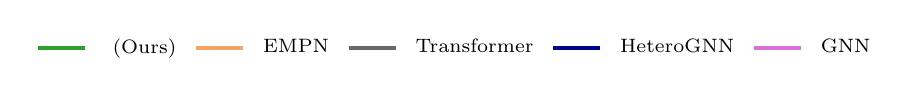
\begin{tikzpicture}
    \tikzstyle{every node}=[font=\scriptsize]
    \definecolor{tabblue}{RGB}{31, 119, 180}
\definecolor{taborange}{RGB}{255, 127, 14}
\definecolor{tabgreen}{RGB}{44, 160, 44}
\definecolor{tabred}{RGB}{214, 39, 40}
\definecolor{tabpurple}{RGB}{148, 103, 189}
\definecolor{tabbrown}{RGB}{140, 86, 75}
\definecolor{tabpink}{RGB}{227, 119, 194}
\definecolor{tabgray}{RGB}{127, 127, 127}
\definecolor{tabolive}{RGB}{188, 189, 34}
\definecolor{tabcyan}{RGB}{23, 190, 207}
\definecolor{lightblue}{RGB}{173, 216, 230}
\definecolor{sandybrown}{RGB}{244, 164, 96}
\definecolor{darkgrey}{RGB}{169, 169, 169}
\definecolor{dimgrey}{RGB}{105, 105, 105}
\definecolor{olivedrab}{RGB}{107, 142, 35}
\definecolor{darkviolet}{RGB}{148, 0, 211}
\definecolor{darkgoldenrod}{RGB}{184, 134, 11}
\definecolor{darkblue}{RGB}{0, 0, 139}
\definecolor{orchid}{RGB}{218, 112, 214}

    \begin{axis}[%
        hide axis,
        xmin=10,
        xmax=50,
        ymin=0,
        ymax=0.1,
        legend style={
            draw=white!15!black,
            legend cell align=left,
            legend columns=5,
            legend style={
                draw=none,
                column sep=1ex,
                line width=1pt,
            }
        },
        ]
        \addlegendimage{line legend, tabgreen, ultra thick} % Thicker line here
        \addlegendentry{\textbf{\model} (Ours)}
        \addlegendimage{line legend, sandybrown, ultra thick} % Thicker line here
        \addlegendentry{EMPN}
        \addlegendimage{line legend, dimgrey, ultra thick} % Thicker line here
        \addlegendentry{Transformer}
        \addlegendimage{line legend, darkblue, ultra thick} % Thicker line here
        \addlegendentry{HeteroGNN}
        \addlegendimage{line legend, orchid, ultra thick} % Thicker line here
        \addlegendentry{GNN}
    \end{axis}
\end{tikzpicture}

    }
    \centering
    % First row of figures
    \begin{subfigure}[b]{0.32\linewidth}
        \includegraphics[width=\textwidth]{ICLR_2025/Figures/eval_cloth_hanging_equi/eval_full_Isaac-Cloth-Hanging-Multi-v0_eval_all.pdf}
        \caption{}
    \end{subfigure}
    \hfill
    \begin{subfigure}[b]{0.32\linewidth}
        \includegraphics[width=\textwidth]{ICLR_2025/Figures/eval_cloth_hanging_equi/eval_half_yaw_Isaac-Cloth-Hanging-Multi-v0_eval_all.pdf}
        \caption{}
    \end{subfigure}
    \hfill
    \begin{subfigure}[b]{0.32\linewidth}
        \includegraphics[width=\textwidth]{ICLR_2025/Figures/eval_cloth_hanging_equi/eval_quater_yaw_Isaac-Cloth-Hanging-Multi-v0_eval_all.pdf}
        \caption{}
    \end{subfigure}
    
    \medskip
    % Second row of figures - centered by wrapping in a minipage
    \begin{minipage}{0.65\textwidth}
    \centering
    \begin{subfigure}[b]{0.49\linewidth}
        \includegraphics[width=\textwidth]{ICLR_2025/Figures/eval_cloth_hanging_equi/appx_eval_quater_half_yaw_Isaac-Cloth-Hanging-Multi-v0_eval_all.pdf}
        \caption{}
    \end{subfigure}
    \hfill
    \begin{subfigure}[b]{0.49\linewidth}
        \includegraphics[width=\textwidth]{ICLR_2025/Figures/eval_cloth_hanging_equi/appx_eval_one_yaw_Isaac-Cloth-Hanging-Multi-v0_eval_all.pdf}
        \caption{}
    \end{subfigure}
    \end{minipage}
    \caption{Performance of different models on the \emph{Cloth-Hanging} task across various sample spaces. Assuming the global scene located at $r=[0,1,0]^T$, then from left to right, we generate sample by rotating $r$ by (a) $\theta_{\text{roll}} \in (-\pi/4, \pi/2)$, $\theta_{\text{yaw}} \in (-\pi, \pi)$, (b) $\theta_{\text{yaw}} \in (-\pi/2, \pi/2)$, and (c) $\theta_{\text{yaw}} \in (-\pi/4, \pi/4)$. Meanwhile, the bottom row shows results for (d) $\theta_{\text{yaw}}\in (-\pi/8, \pi/8)$, and (e) the fixed orientation at $\theta_{\text{roll}}=0, \theta_{\text{yaw}}=0$. As the sample space decreases, performance improves across all models, with HEPi consistently outperforming the baselines. The additional plot with fixed orientation on the bottom are averaged over 5 seeds while the others with 10 seeds.}
    \vspace{-0.2cm}
    \label{fig:appx_eval_equi}
\end{figure*}

\paragraph{Ablation on smaller sample space}

Here, we show a more detail version of the ablation in Figure~\ref{fig:eval_equi}. In addition to different sample spaces in the main paper, we evaluate all the methods on the scenarios when drawing $\theta_{\text{yaw}} \in (-\pi/8, \pi/8)$ and with a fixed-angle setting at $\theta_{\text{roll}} = 0, \theta_{\text{yaw}} = 0$. 

As shown in Figure~\ref{fig:appx_eval_equi}, performance generally increases as the orientation range narrows. Interestingly, HeteroGNN performs better than its non-heterogeneous GNN in most cases, showing its high expressiveness though being less sample efficient. This phenomenon can be attributed to the shared networks among all the edge types of the naive GNN model. However, once employing EMPN as the backbone, \model consistently outperforms all the baselines in terms of both the performance and sample effeciency. This proves equivariant constraint plays a crucial role to reduce the problem complexity in large 3D space.

\paragraph{Ablation on K-NN for obj-to-act edges}

\begin{figure*}[t]
    \centering
    \hfill
    \begin{subfigure}[b]{0.32\linewidth}
        \includegraphics[width=\textwidth]{ICLR_2025/Figures/appx_theory/appx_eval_knn_vn_m2_Isaac-Rigid-Insertion-Multi-v0_eval_all.pdf}
        % \caption{$m=2$} 
    \end{subfigure}
    \hfill
    \begin{subfigure}[b]{0.32\linewidth}
        \includegraphics[width=\textwidth]{ICLR_2025/Figures/appx_theory/appx_eval_knn_vn_m2_Isaac-Rigid-Insertion-Multi-Two-Actuators-v0_eval_all.pdf}
        % \caption{$m=3$}
    \end{subfigure}
    \hfill
    \begin{subfigure}[b]{0.32\linewidth}
        \includegraphics[width=\textwidth]{ICLR_2025/Figures/appx_theory/appx_eval_knn_vn_m2_Isaac-Rope-Shaping-v0_eval_all.pdf}
        % \caption{$m=4$}
    \end{subfigure}
    \hfill
    \caption{Ablation on different $k$-nearest neighbors choices for \textit{obj-to-act} edges in $\text{MPNN}$ + $\text{VN}_{\text {Local}}$ updates (in Section~\ref{sec:main_theorem}), evaluated across multiple tasks: \textit{rigid-insertion}, \textit{rigid-insertion-two-agents}, and \textit{rope-shaping}. Results are averaged over 8 seeds.}
    \vspace{-0.2cm}
    \label{fig:appx_knn_vn_num_mess0}
\end{figure*}


Ablation in Figure \ref{fig:appx_knn_vn_num_mess0} investigates the update of $\text{MPNN}$ + $\text{VN}_{\text {Local}} $ with varying k-nearest neighbors on tasks \textit{rigid-insertion}, \textit{rigid-insertion-two-agents} and \textit{rope-shaping}. For the two insertion tasks, the maximum node size is 25; therefore, we only vary $k$ from $1$ to $10$. On the other hand, \textit{rope-shaping} task has $80$ nodes, so $k$ is picked from $\{1, 10, 20, 50\}$. As shown, when $k$ is small, there are no-overlapping nodes, the actuator nodes can miss the information from distant nodes. Meanwhile, when $k$ is bigger, the number of overlapping nodes increase, and therefore, these nodes can be reached after one layer of message passing, thus resulting in higher expected return.

\begin{figure*}[htb]
    \makebox[\textwidth][c]{
    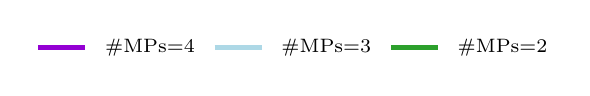
\begin{tikzpicture}
    \tikzstyle{every node}=[font=\scriptsize]
    \definecolor{tabblue}{RGB}{31, 119, 180}
\definecolor{taborange}{RGB}{255, 127, 14}
\definecolor{tabgreen}{RGB}{44, 160, 44}
\definecolor{tabred}{RGB}{214, 39, 40}
\definecolor{tabpurple}{RGB}{148, 103, 189}
\definecolor{tabbrown}{RGB}{140, 86, 75}
\definecolor{tabpink}{RGB}{227, 119, 194}
\definecolor{tabgray}{RGB}{127, 127, 127}
\definecolor{tabolive}{RGB}{188, 189, 34}
\definecolor{tabcyan}{RGB}{23, 190, 207}
\definecolor{lightblue}{RGB}{173, 216, 230}
\definecolor{sandybrown}{RGB}{244, 164, 96}
\definecolor{darkgrey}{RGB}{169, 169, 169}
\definecolor{dimgrey}{RGB}{105, 105, 105}
\definecolor{olivedrab}{RGB}{107, 142, 35}
\definecolor{darkviolet}{RGB}{148, 0, 211}
\definecolor{darkgoldenrod}{RGB}{184, 134, 11}
\definecolor{darkblue}{RGB}{0, 0, 139}
\definecolor{orchid}{RGB}{218, 112, 214}

    \begin{axis}[%
        hide axis,
        xmin=10,
        xmax=50,
        ymin=0,
        ymax=0.1,
        legend style={
            draw=white!15!black,
            legend cell align=left,
            legend columns=3,
            legend style={
                draw=none,
                column sep=1ex,
                line width=1pt,
            }
        },
        ]
        \addlegendimage{line legend, darkviolet, ultra thick} % Thicker line here
        \addlegendentry{\#MPs=4}
        \addlegendimage{line legend, lightblue, ultra thick} % Thicker line here
        \addlegendentry{\#MPs=3}
        \addlegendimage{line legend, tabgreen, ultra thick} % Thicker line here
        \addlegendentry{\#MPs=2}
    \end{axis}
\end{tikzpicture}

    }
    \centering
    \begin{subfigure}[b]{0.32\linewidth}
        \includegraphics[width=\textwidth]{ICLR_2025/Figures/appx_eval_num-mess/new_appx_num-mess_dim_eval_bar_Isaac-Rigid-Insertion-Multi-v0_eval_consistent.pdf}
    \end{subfigure}
    \hfill
    \begin{subfigure}[b]{0.32\linewidth}
        \includegraphics[width=\textwidth]{ICLR_2025/Figures/appx_eval_num-mess/new_appx_num-mess_dim_eval_bar_Isaac-Rigid-Insertion-Multi-Two-Actuators-v0_eval_consistent.pdf}
    \end{subfigure}
    \hfill
    \begin{subfigure}[b]{0.32\linewidth}
        \includegraphics[width=\textwidth]{ICLR_2025/Figures/appx_eval_num-mess/new_appx_num-mess_dim_eval_bar_Isaac-Cloth-Hanging-Multi-v0_eval_all.pdf}
    \end{subfigure}
    \caption{Ablation on the number of message-passing steps (\#MPs) for HEPi and EMPN models. For HEPi, \#MPs=$m$ refers to $m-1$ object-to-object message-passing layers. Across all tasks, increasing the number of message-passing steps beyond a certain point does not improve performance, as the proposed graph design already efficiently transmits information from observations to actions. Results are averaged over 5 seeds.}
    \vspace{-0.2cm}
    \label{fig:appx_mp_ablation}
\end{figure*}


\begin{figure*}[t]
    \makebox[\textwidth][c]{
    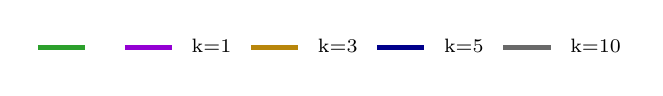
\begin{tikzpicture}
    \tikzstyle{every node}=[font=\scriptsize]
    \definecolor{tabblue}{RGB}{31, 119, 180}
\definecolor{taborange}{RGB}{255, 127, 14}
\definecolor{tabgreen}{RGB}{44, 160, 44}
\definecolor{tabred}{RGB}{214, 39, 40}
\definecolor{tabpurple}{RGB}{148, 103, 189}
\definecolor{tabbrown}{RGB}{140, 86, 75}
\definecolor{tabpink}{RGB}{227, 119, 194}
\definecolor{tabgray}{RGB}{127, 127, 127}
\definecolor{tabolive}{RGB}{188, 189, 34}
\definecolor{tabcyan}{RGB}{23, 190, 207}
\definecolor{lightblue}{RGB}{173, 216, 230}
\definecolor{sandybrown}{RGB}{244, 164, 96}
\definecolor{darkgrey}{RGB}{169, 169, 169}
\definecolor{dimgrey}{RGB}{105, 105, 105}
\definecolor{olivedrab}{RGB}{107, 142, 35}
\definecolor{darkviolet}{RGB}{148, 0, 211}
\definecolor{darkgoldenrod}{RGB}{184, 134, 11}
\definecolor{darkblue}{RGB}{0, 0, 139}
\definecolor{orchid}{RGB}{218, 112, 214}

    \begin{axis}[%
        hide axis,
        xmin=10,
        xmax=50,
        ymin=0,
        ymax=0.1,
        legend style={
            draw=white!15!black,
            legend cell align=left,
            legend columns=5,
            legend style={
                draw=none,
                column sep=1ex,
                line width=1pt,
            }
        },
        ]
        \addlegendimage{line legend, tabgreen, ultra thick} % Thicker line here
        \addlegendentry{\textbf{\model}}
        \addlegendimage{line legend, darkviolet, ultra thick} % Thicker line here
        \addlegendentry{k=1}
        \addlegendimage{line legend, darkgoldenrod, ultra thick} % Thicker line here
        \addlegendentry{k=3}
        \addlegendimage{line legend, darkblue, ultra thick} % Thicker line here
        \addlegendentry{k=5}
        \addlegendimage{line legend, dimgrey, ultra thick} % Thicker line here
        \addlegendentry{k=10}
        
    \end{axis}
\end{tikzpicture}

    }
    \centering
    \hfill
    \begin{subfigure}[b]{0.32\linewidth}
        \includegraphics[width=\textwidth]{ICLR_2025/Figures/appx_theory/eval_knn_vn_m2_Isaac-Rigid-Insertion-Multi-v0_eval_all.pdf}
        \caption{$m=1$} 
    \end{subfigure}
    \hfill
    \begin{subfigure}[b]{0.32\linewidth}
        \includegraphics[width=\textwidth]{ICLR_2025/Figures/appx_theory/eval_knn_vn_m3_Isaac-Rigid-Insertion-Multi-v0_eval_all.pdf}
        \caption{$m=2$}
    \end{subfigure}
    \hfill
    \begin{subfigure}[b]{0.32\linewidth}
        \includegraphics[width=\textwidth]{ICLR_2025/Figures/appx_theory/eval_knn_vn_m4_Isaac-Rigid-Insertion-Multi-v0_eval_all.pdf}
        \caption{$m=3$}
    \end{subfigure}
    \hfill
    \caption{Ablation on different $k$-nearest neighbors for \textit{obj-to-act} edges in $\text{MPNN}$ + $\text{VN}_{\text {Local}}$ (in Section~\ref{sec:main_theorem}) updates, evaluated on the \emph{Rigid-Insertion} task with varying message passing steps \update{$m \in \{1,2,3\}$ for object nodes}. Increasing the number of message passing steps degrades performance due to oversquashing. Results are averaged over 5 seeds.}

    \vspace{-0.2cm}
    \label{fig:appx_knn_vn_num_mess}
\end{figure*}


\paragraph{Ablation on Number of Message-Passing Steps}

In this ablation, we examine the impact of varying the number of message-passing steps (\#MPs) in both HEPi and a naive EMPN model. Our goal is to determine whether increasing the number of message-passing steps improves policy learning.

As shown in Figure~\ref{fig:appx_mp_ablation}, increasing the number of message-passing steps does not yield significant improvements. Moreover, Figure~\ref{fig:appx_knn_vn_num_mess} specifically demonstrates that increasing number of message passing can lead to oversquashing, where the amount of information exponentially decays by the number of hops, and hence lead to performance drop. HEPi, on the other hand, efficiently reduces the information transmission time to only one hop. These results suggest that, in our design, fewer message-passing steps suffice to capture the necessary information flow, reinforcing the efficiency of our graph design.


\begin{figure*}[h]
    \makebox[\textwidth][c]{
    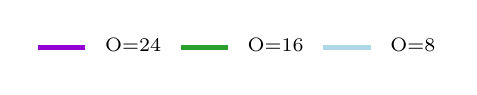
\begin{tikzpicture}
    \tikzstyle{every node}=[font=\scriptsize]
    \definecolor{tabblue}{RGB}{31, 119, 180}
\definecolor{taborange}{RGB}{255, 127, 14}
\definecolor{tabgreen}{RGB}{44, 160, 44}
\definecolor{tabred}{RGB}{214, 39, 40}
\definecolor{tabpurple}{RGB}{148, 103, 189}
\definecolor{tabbrown}{RGB}{140, 86, 75}
\definecolor{tabpink}{RGB}{227, 119, 194}
\definecolor{tabgray}{RGB}{127, 127, 127}
\definecolor{tabolive}{RGB}{188, 189, 34}
\definecolor{tabcyan}{RGB}{23, 190, 207}
\definecolor{lightblue}{RGB}{173, 216, 230}
\definecolor{sandybrown}{RGB}{244, 164, 96}
\definecolor{darkgrey}{RGB}{169, 169, 169}
\definecolor{dimgrey}{RGB}{105, 105, 105}
\definecolor{olivedrab}{RGB}{107, 142, 35}
\definecolor{darkviolet}{RGB}{148, 0, 211}
\definecolor{darkgoldenrod}{RGB}{184, 134, 11}
\definecolor{darkblue}{RGB}{0, 0, 139}
\definecolor{orchid}{RGB}{218, 112, 214}

    \begin{axis}[%
        hide axis,
        xmin=10,
        xmax=50,
        ymin=0,
        ymax=0.1,
        legend style={
            draw=white!15!black,
            legend cell align=left,
            legend columns=3,
            legend style={
                draw=none,
                column sep=1ex,
                line width=1pt,
            }
        },
        ]
        \addlegendimage{line legend, darkviolet, ultra thick} % Thicker line here
        \addlegendentry{O=24}
        \addlegendimage{line legend, tabgreen, ultra thick} % Thicker line here
        \addlegendentry{O=16}
        \addlegendimage{line legend, lightblue, ultra thick} % Thicker line here
        \addlegendentry{O=8}
    \end{axis}
\end{tikzpicture}

    }
    \centering
    \begin{subfigure}[b]{0.32\linewidth}
        % \includegraphics[width=\textwidth]{ICLR_2025/Figures/appx_eval_ori/appx_ori_dim_eval_bar_Isaac-Rigid-Insertion-Multi-v0_eval_consistent.pdf}
        \includegraphics[width=\textwidth]{ICLR_2025/Figures/appx_eval_ori/new_appx_ori_dim_eval_bar_Isaac-Rigid-Insertion-Multi-v0_eval_consistent.pdf}
    \end{subfigure}
    \hfill
    \begin{subfigure}[b]{0.32\linewidth}
        % \includegraphics[width=\textwidth]{ICLR_2025/Figures/appx_eval_ori/appx_ori_dim_eval_bar_Isaac-Rigid-Insertion-Multi-Two-Actuators-v0_eval_consistent.pdf}
        \includegraphics[width=\textwidth]{ICLR_2025/Figures/appx_eval_ori/new_appx_ori_dim_eval_bar_Isaac-Rigid-Insertion-Multi-Two-Actuators-v0_eval_consistent.pdf}
    \end{subfigure}
    \hfill
    \begin{subfigure}[b]{0.32\linewidth}
        % \includegraphics[width=\textwidth]{ICLR_2025/Figures/appx_eval_ori/appx_ori_dim_eval_bar_Isaac-Cloth-Hanging-Multi-v0_eval_all.pdf}
        \includegraphics[width=\textwidth]{ICLR_2025/Figures/appx_eval_ori/new_appx_ori_dim_eval_bar_Isaac-Cloth-Hanging-Multi-v0_eval_all.pdf}
    \end{subfigure}
    \caption{Ablation on the orientation discretization dimension (\texttt{ori\_dim}). Increasing \texttt{ori\_dim} improves performance in 3D tasks, such as \textit{rigid-insertion} and \textit{cloth-hanging}, by better approximating full equivariance. However, higher \texttt{ori\_dim} also increases training time. Results are averaged over 5 seeds.}
    \vspace{-0.2cm}
    \label{fig:appx_ori_dim}
\end{figure*}


\paragraph{Ablation on Orientation Discretization (ori\_dim)}

In this ablation, we explore the impact of varying the orientation discretization dimension (\texttt{ori\_dim}) in the Equivariant Message Passing Network (EMPN). The \texttt{ori\_dim} controls how finely we sample orientations from the $S^2$ sphere, where a higher \texttt{ori\_dim} increases the number of samples and better approximates full equivariance. In our main experiments, we used a default \texttt{ori\_dim} of 16. Here, we vary \texttt{ori\_dim} across 8, 16, and 24.

As shown in Figure~\ref{fig:appx_ori_dim}, increasing \texttt{ori\_dim} generally improves performance in 3D tasks, as a finer discretization better captures orientation changes. However, this comes at the cost of increased training time due to the higher computational demand. Notably, in simpler 2D tasks, increasing \texttt{ori\_dim} does not significantly affect performance, so we focus on 3D tasks for this ablation.


\begin{figure*}[htb]
    \centering
    \begin{subfigure}[b]{0.24\linewidth}
        \includegraphics[width=\textwidth]{ICLR_2025/Figures/appx_eval_knn/new_appx_consitent_knn_eval_bar_Isaac-Rigid-Sliding-Multi-v0_eval_all.pdf}
    \end{subfigure}
    \hfill
    \begin{subfigure}[b]{0.24\linewidth}
        \includegraphics[width=\textwidth]{ICLR_2025/Figures/appx_eval_knn/appx_knn_eval_bar_Isaac-Rigid-Insertion-Multi-v0_eval_consistent.pdf}
    \end{subfigure}
    \hfill
    \begin{subfigure}[b]{0.24\linewidth}
        \includegraphics[width=\textwidth]{ICLR_2025/Figures/appx_eval_knn/appx_knn_eval_bar_Isaac-Rigid-Insertion-Multi-Two-Actuators-v0_eval_consistent.pdf}
    \end{subfigure}
    \hfill
    \begin{subfigure}[b]{0.24\linewidth}
        \includegraphics[width=\textwidth]{ICLR_2025/Figures/appx_eval_knn/appx_knn_eval_bar_Isaac-Rope-Shaping-v0_eval_all.pdf}
    \end{subfigure}
    \caption{Ablation on the number of nearest neighbors (\texttt{KNN\_k}) used in the KNN graph on HEPi. Increasing \texttt{KNN\_k} beyond 3 does not improve performance and may even reduce it, particularly in tasks like \textit{rope-shaping-2D}, due to message overcapacity. Results are averaged over 5 seeds.}

    \vspace{-0.2cm}
    \label{fig:appx_knn_k}
\end{figure*}


\paragraph{Ablation on K-Nearest Neighbor Graph (KNN\_k)}

In this ablation, we evaluate the effect of varying the number of nearest neighbors (\texttt{KNN\_k}) used to connect object nodes in our graph. Instead of relying on mesh edges, we use a K-nearest neighbor (KNN) graph to ensure a more generic representation, a common practice in PointCloud-based representations.

As shown in Figure~\ref{fig:appx_knn_k}, our default setting of \texttt{KNN\_k=3} performs comparably to higher values of \texttt{KNN\_k}. Increasing the number of nearest neighbors does not provide additional benefits and can even degrade performance slightly, as seen in the \textit{rope-shaping-2D} task. This is likely due to the overcapacity of messages being passed through the network, which introduces unnecessary complexity in the message aggregation process.

\section{Evaluation Details}
\label{appx:eval_details}
\subsection{Implementation Details}

All experiments were conducted on a machine equipped with an NVIDIA A100 or an NVIDIA H100 GPU. We utilized the TorchRL framework \citep{bou2023torchrl} for the implementation of PPO and TRPL algorithms, and PyG (PyTorch Geometric) \citep{pyg} for handling the graph-based structure. The Transformer architecture was implemented using the \texttt{torch.nn.TransformerEncoder} and \texttt{torch.nn.TransformerEncoderLayer} packages from PyTorch \citep{torch}.

\subsection{Computational Time}

We report the computational time for each model on all tasks here. Table~\ref{tab:compute-time} reports the total training time and Table~\ref{tab:num-max-nodes} demonstrates the size of the input graph, which is the main factor contributing to the total training time.

\begin{table}[htb]
\centering
\caption{Total training time for each task (in hours). (*) We note that the fast training speed of Transformer might be attributed to the internal optimization implementation of \texttt{PyTorch}. (**) In \textit{Rope-Shaping} task, we report the training time on NVIDIA H100 GPU.}
\label{tab:compute-time}
\begin{adjustbox}{max width=\textwidth}
\begin{tabular}{lccc}
\toprule
    & \textbf{HEPi} & \textbf{EMPN} & $\textbf{Transformer}^*$ \\ 
\midrule
\multicolumn{4}{l}{} \\
Rigid-Sliding                  & 2h 10m         & 2h 56m         & 1h 15m  \\
\rebuttal{Rigid-Pushing}       & \rebuttal{2h 58m}         & \rebuttal{3h 58m}         & \rebuttal{1h 52m}  \\
Rigid-Insertion                & 1h 56m         & 2h 35m         & 1h 14m \\
Rigid-Insertion-Two-Agents     & 1h 3m          & 1h 20m         & 36m  \\
Rope-Closing                   & 1h 14m         & 1h 40m         & 51m  \\
$\text{Rope-Shaping}^{**}$     & 2h 58m         & 4h 57m         & 1h 56m  \\
Cloth-Hanging                  & 2h 40m         & 2h 36m         & 2h 21m  \\
\bottomrule
\end{tabular}
\end{adjustbox}
\end{table}

\begin{table}[htb]
\centering
\caption{Maximum number of nodes and type of connection for each task.}
\label{tab:num-max-nodes}
\begin{adjustbox}{max width=\textwidth}
\begin{tabular}{lcc}
\toprule
\textbf{Shape} & \textbf{Maximum \#nodes} & \textbf{Graph Connections} \\ 
\midrule
Rigid-Sliding                  & 25   & knn=3 \\
Rigid-Insertion                & 25   & knn=3 \\
Rigid-Pushing                  & 25   & knn=3 \\
Rigid-Insertion-Two-Agents     & 25   & knn=3 \\
Rope-Closing                   & 40   & knn=3 \\
Rope-Shaping                   & 80   & knn=3 \\
Cloth-Hanging                  & 10   & complete \\
\bottomrule
\end{tabular}
\end{adjustbox}
\end{table}

\subsection{Grid Search for PPO}
\label{sec:appx_grid_search_ppo}

To fairly compare PPO with TRPL, we perform a grid search for PPO over 5 seeds and select the best-performing configuration based on the maximum return. We then run the chosen configuration on 5 additional seeds and report the results in Figure~\ref{fig:eval_trpl_ppo}. Specifically, we tune the \texttt{clip\_eps} parameter, which controls how much the new policy is allowed to deviate from the old policy, with values \{0.1, 0.2, 0.3, 0.5\}, and explore both with and without annealing (\texttt{anneal\_clip\_eps=True or False}). The \texttt{clip\_eps} bounds the probability ratio between the new and old policies to \((1 - \epsilon, 1 + \epsilon)\), preventing large updates and ensuring stable learning. Lower values of \texttt{clip\_eps} result in more conservative updates, while higher values allow more flexibility in policy updates. Annealing progressively decreases \texttt{clip\_eps} over time, tightening the constraint as training progresses.

\subsection{Hyperparameters}

We presents the hyperparameters used across all policy models (HEPi, EMPN, and Transformer) for all the tasks in Table~\ref{tab:model-HP}.

\begin{table}[ht]
\centering
\caption{Hyperparameters used for all tasks. In EMPN, the number of layers (*) corresponds to the number of message-passing steps.}
\label{tab:model-HP}
\begin{adjustbox}{max width=\textwidth}
\begin{tabular}{lccc}
\toprule
    & \textbf{HEPi} & \textbf{EMPN} & \textbf{Transformer} \\ 
\midrule
\multicolumn{4}{l}{} \\
contextual std                   & true         & true        & true \\
latent dim.                      & 64           & 64          & 64 \\
activation                       & GELU         & GELU        & ReLU \\
dropout                          & false        & false       & false \\
num layers                       & n.a.         & $\text{2}^*$          & 2 \\
num heads                        & n.a.         & n.a.        & 2 \\
num messages (obj-to-obj)        & 1            & n.a.        & n.a. \\
num messages (obj-to-act)        & 1            & n.a.        & n.a. \\
num messages (act-to-act)        & 1            & n.a.        & n.a. \\
ponita orientation dim.          & 16           & 16          & n.a. \\
ponita degree                    & 2            & 2           & n.a. \\
ponita spatial hidden dim.       & [64, 64]     & [64, 64]    & n.a. \\
ponita fiber hidden dim.         & [64, 64]     & [64, 64]    & n.a. \\
ponita widening factor           & 4            & 4           & n.a. \\ 
\bottomrule
\end{tabular}
\end{adjustbox}
\end{table}


The following tables, Table~\ref{tab:rigid-HP} and Table~\ref{tab:deformable-HP} provide details on environment settings, data collection parameters, and training hyperparameters.

\begin{table}[htb]
\centering
\caption{Hyperparameters for Rigid Environments}
\label{tab:rigid-HP}
\begin{adjustbox}{max width=\textwidth}
\begin{tabular}{lccc}
\toprule
   & \rebuttal{\textbf{Rigid-Sliding}} & \textbf{Rigid-Insertion} & \textbf{Rigid-Insertion} \\ 
   &                        &       \textbf{ \slash \space Rigid-Pushing}                   & \textbf{-Two-Agents} \\     
\midrule
\multicolumn{4}{l}{} \\
\textbf{Environments}  &             &             &             \\  
time steps             & 100         & 100         & 100            \\ 
warmup steps           & 5           & 5           & 5               \\
episode length (in sec.) & 4           & 4           & 4              \\
decimation             & 4           & 4           & 4               \\
simulation $dt$        & 0.01        & 0.01        & 0.01               \\ 
\midrule
\textbf{Data Collection}  &          &             &             \\  
frames per batch       & 100k        & 100k        & 100k            \\ 
total frames           & 20M         & 20M \slash \space 30M         & 6M             \\
\midrule
\textbf{Input Graph}   &             &             &             \\
obj-to-obj edges       & knn=3       & knn=3       & knn=3     \\
act-to-act edges       & n.a.        & n.a.        & complete    \\
\midrule
\textbf{Training}      &             &             &             \\
epochs                 & 5           & 5           & 5            \\ 
mini-batch size        & 1000        & 1000        & 1000            \\ 
learning rate (actor)  & 3e-4        & 3e-4        & 3e-4             \\
learning rate (critic) & 3e-4        & 3e-4        & 3e-4             \\ 
critic coeff.          & 0.5         & 0.5         & 0.5             \\ 
entropy coeff.         & \rebuttal{0.005}      & 0.005       & 0.005             \\ 
clip gradient norm     & false       & false       & false             \\
\textbf{Projection}    &             &             &             \\
trust region coeff.    & \rebuttal{4.0}         & 1.0         & 1.0              \\ 
mean bound             & 0.05        & 0.05        & 0.05             \\ 
covariant bound        & \rebuttal{0.001}       & 0.0025      & 0.0025             \\
\midrule
\textbf{Critic (DeepSets)}                  &              &             & \\ 
num inner layers                 & 2         & 2          & 2 \\
num outer layers                 & 2         & 2          & 2 \\
hidden dim.                      & 64           & 64          & 64 \\
activation                       & ReLU         & ReLU        & ReLU \\
layer norm                       & true         & true        & true  \\ 
\bottomrule
\end{tabular}
\end{adjustbox}
\end{table}

\begin{table}[htb]
\centering
\caption{Hyperparameters for Deformable Environments}
\label{tab:deformable-HP}
\begin{adjustbox}{max width=\textwidth}
\begin{tabular}{lccc}
\toprule
   & \textbf{Rope-Closing} & \textbf{Rope-Shaping} & \textbf{Cloth-Hanging} \\ 
\midrule
\multicolumn{4}{l}{} \\
\textbf{Environments}  &             &             &             \\  
time steps             & 200          & 200          & 100          \\ 
warmup steps           & 10           & 10           & 10           \\
episode length (in sec.) & 4           & 4           & 2            \\
decimation             & 2           & 2           & 2               \\
simulation $dt$        & 0.01        & 0.01        & 0.01               \\ 
\midrule
\textbf{Data Collection}  &             &             &             \\
frames per batch       & 40k          & 40k          & 10k          \\ 
total frames           & 4M           & 10M          & 5M           \\
\midrule
\textbf{Input Graph}   &             &             &             \\
obj-to-obj edges       & knn=3        & knn=3       & complete \\
act-to-act edges       & complete     & complete    & complete  \\
\midrule
\textbf{Training}      &             &             &             \\
epochs                 & 5           & 5           & 5            \\ 
mini-batch size        & 200          & 200          & 200            \\ 
learning rate (actor)  & 3e-4        & 3e-4        & 3e-4             \\
learning rate (critic) & 3e-4        & 3e-4        & 3e-4             \\ 
critic coeff.          & 0.5         & 0.5         & 0.5             \\ 
entropy coeff.         & 0.005       & 0.005       & 0.005             \\ 
clip gradient norm     & false       & false       & false             \\ 
\textbf{Projection}    &             &             &                \\
trust region coeff.    & 4.0         & 1.0         & 4.0              \\ 
mean bound             & 0.05        & 0.05        & 0.05             \\ 
covariant bound        & 0.001       & 0.0025      & 0.001             \\
\midrule
\textbf{Critic (DeepSets)}                  &              &             & \\ 
num inner layers                 & 2         & 2          & 2 \\
num outer layers                 & 2         & 2          & 2 \\
hidden dim.                      & 64           & 64          & 64 \\
activation                       & ReLU         & ReLU        & ReLU \\
layer norm                       & true         & true        & true  \\ 
\bottomrule
\end{tabular}
\end{adjustbox}
\end{table}

